
\documentclass[journal]{IEEEtran}
\usepackage{graphicx}
\begin{document}
\title{De Bruijn Graphs, Sheaf Structures, Homology, and Coding Theory}
\author{R.A. Posthumus}
\maketitle

\section{Figures}
\begin{figure}[h]
\centering
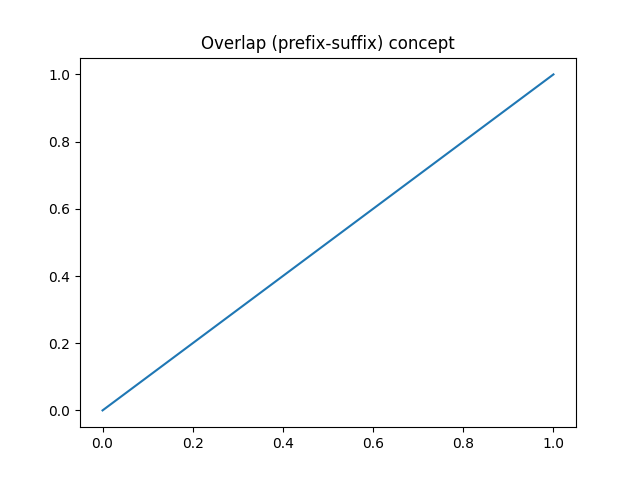
\includegraphics[width=0.4\linewidth]{figure_overlap.png}
\caption{Overlap locality}
\end{figure}

\begin{figure}[h]
\centering

\includegraphics[width=0.4\linewidth]{figure_sheaf.png}
\caption{Sheaf gluing}
\end{figure}

\begin{figure}[h]
\centering
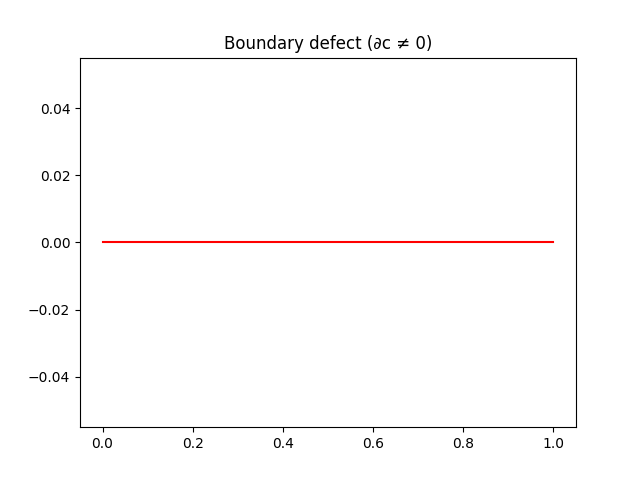
\includegraphics[width=0.4\linewidth]{figure_boundary.png}
\caption{Boundary defect}
\end{figure}

\end{document}
